\chapter{Метод интеллектуальной поддержки принятия решений оптимального размещения объектов обслуживания на основе оптимизации транспортной сети}
\label{ch:decision-support-method}

\section{Математическая постановка задачи оптимального размещения}
\label{sec:optimal-placement-statement}


\begin{figure}
    \centering
    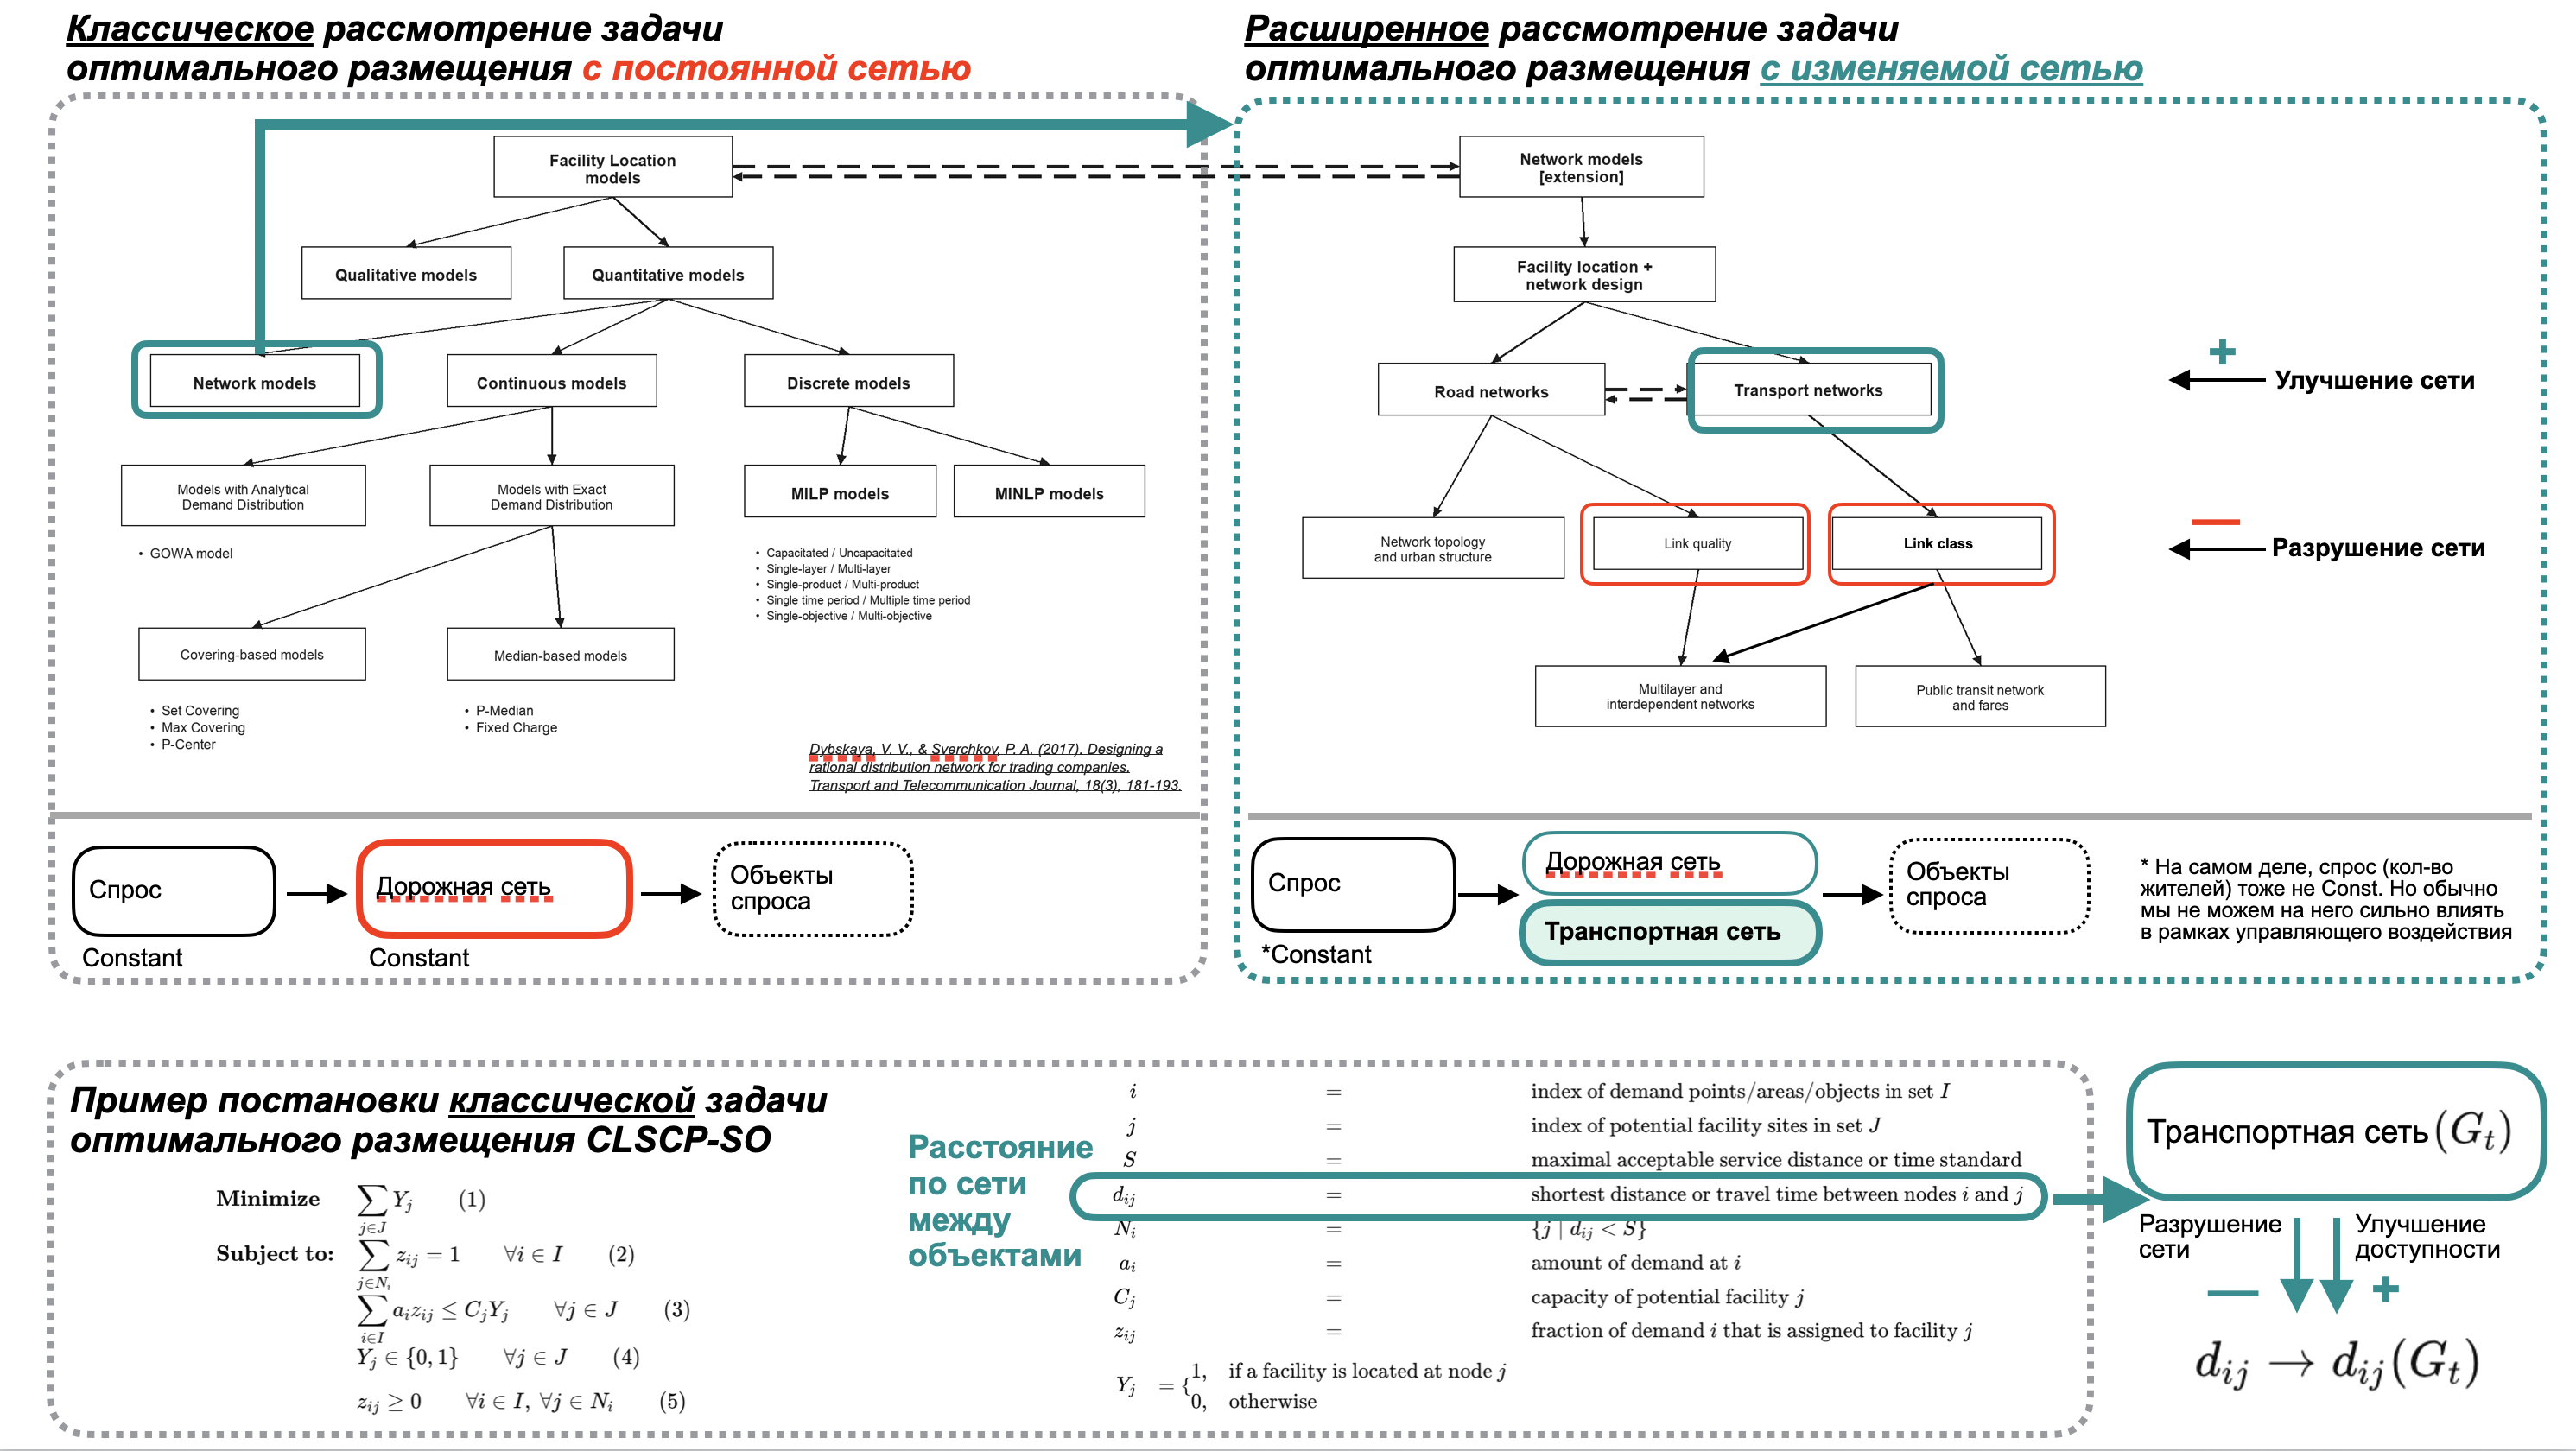
\includegraphics[width=1\linewidth]{images/3}
    \caption{Расширение задачи об оптимальном размещении с учетом изменений состояний транспортной сети.}
    \label{fig:3}
\end{figure}

\subsection{Интегрированная задача размещения и дорожного строительства}
\label{subsec:chapter3-daskin}

В работе \cite{daskin1993towardIntegrated,melkote1996integrated,melkote2001integrated}
рассматривается смешанно-целочисленная постановка неемкостной задачи совместного размещения объектов и проектирования сети.
Пусть
$N$ --- множество узлов,
$L$ --- множество кандидатных дорожных ребер,
$d_i$ --- спрос в узле $i$,
$f_i$ --- стоимость открытия объекта в узле $i$,
$c_{ij}$ --- стоимость строительства ребра $(i,j)$,
$t_{ij}$ --- транспортная стоимость единицы потока по ребру $(i,j)$,
$M=\sum_{i\in N} d_i$ --- суммарный спрос сети.

Переменные модели:
\[
Z_i =
\begin{cases}
1, & \text{если объект открыт в узле } i,\\
0, & \text{иначе},
\end{cases}
\]
\[
X_{ij} =
\begin{cases}
1, & \text{если дорожное ребро } (i,j) \text{ строится},\\
0, & \text{иначе},
\end{cases}
\]
\[
Y_{ij},\,Y_{ji} \ge 0 \text{ --- поток спроса по ребру } (i,j) \text{ в двух направлениях}.
\]
\[
W_i \ge 0 \text{ --- спрос, обслуженный объектом в узле } i.
\]

Тогда задача записывается как
\[
\min
\sum_{(i,j)\in L} t_{ij}(Y_{ij}+Y_{ji})
+ \sum_{i\in N} f_i Z_i
+ \sum_{(i,j)\in L} c_{ij} X_{ij}.
\]

При ограничениях
\[
\sum_{j\in N} Y_{ji} + d_i
=
\sum_{j\in N} Y_{ij} + W_i,
\qquad \forall i\in N,
\]
\[
W_i \le M Z_i,
\qquad \forall i\in N,
\]
\[
Y_{ij} \le M X_{ij}, \qquad
Y_{ji} \le M X_{ij},
\qquad \forall (i,j)\in L,
\]
\[
Z_i \in \{0,1\}, \qquad
X_{ij} \in \{0,1\}.
\]

\subsection{Размещение объектов при изменении транспортной достижимости}
\label{subsec:chapter3-tikhevich}

В работе \cite{kontsevik2024connectivityPlacement} меняется уже не дорожный граф как таковой,
а матрица времен транспортной достижимости между районами.
Пусть
$I$ --- множество районов спроса,
$J$ --- множество районов-кандидатов для размещения сервиса,
$T_{ij}$ --- исходное время достижения из $i$ в $j$,
$S$ --- норматив доступности,
$q_j$ --- емкость сервиса в узле $j$,
$d_i$ --- спрос в узле $i$.

Church и Murray (2018), описывают модель CLSCP-SO следующим образом:
``Разместить ровно столько объектов и связанной с ними мощности, сколько необходимо, чтобы весь спрос был обслужен в пределах ограничений мощности каждого объекта с учетом возможностей покрытия каждого объекта.''

Ниже приводится запись модели в нотации источника:
\[
\begin{array}{rll}
\textbf{Минимизировать}
& \displaystyle \sum_{j\in J} Y_j
& \\[0.4em]
\textbf{При условиях:}
& \displaystyle \sum_{j\in N_i} z_{ij} = 1,
& \forall i\in I, \\[0.8em]
& \displaystyle \sum_{i\in I} a_i z_{ij} \le C_j x_j,
& \forall j\in J, \\[0.8em]
& Y_j \in \{0,1\},
& \forall j\in J, \\[0.4em]
& z_{ij} \ge 0,
& \forall i\in I,\ \forall j\in N_i .
\end{array}
\]

Во втором ограничении сохранена исходная запись источника с $x_j$; в целевой функции, бинарном ограничении и определении ниже тот же индикатор записан как $Y_j$.

Где
\[
\begin{array}{rcl}
i & = & \text{индекс узлов спроса из множества } I, \\
j & = & \text{индекс потенциальных площадок из множества } J, \\
S & = & \text{максимально допустимое время или расстояние обслуживания}, \\
d_{ij} & = & \text{кратчайшее расстояние или время движения между } i \text{ и } j, \\
N_i & = & \{j \mid d_{ij} < S\}, \\
a_i & = & \text{величина спроса в узле } i, \\
C_j & = & \text{емкость потенциального объекта } j, \\
z_{ij} & = & \text{доля спроса } i\text{, назначенная объекту } j, \\
Y_j & = &
\begin{cases}
1, & \text{если объект размещается в узле } j,\\
0, & \text{иначе}.
\end{cases}
\end{array}
\]

В работе \cite{kontsevik2024connectivityPlacement} используется улучшенный алгоритм MCLP --- CLSCP-SO.
При этом матрица стоимости рассматривается как константа; в рассматриваемой постановке
матрица стоимости --- это матрица достижимости между выбранными районами,
которая далее модифицируется относительно числа размещаемых поликлиник.

\begin{table}[h]
    \centering
    \small
    \caption{Пример матрицы транспортной доступности}
    \label{tab:chapter3-tikhevich-toy-matrix}
    \begin{tabular}{c|cccccccccc}
        \textbf{идентификатор блока} & \textbf{0} & \textbf{1} & \textbf{2} & \textbf{3} & \textbf{4} & \textbf{5} & \textbf{6} & \textbf{7} & \textbf{8} & \textbf{9} \\
        \hline
        \textbf{0} & 0.0 & 11.3 & \cellcolor{yellow!25}21.0 & \cellcolor{yellow!25}25.0 & 27.6 & 26.5 & 34.6 & 32.4 & 26.1 & \cellcolor{yellow!25}25.0 \\
        \textbf{1} & 11.3 & 0.0 & \cellcolor{yellow!25}24.5 & 27.3 & 29.9 & 28.8 & 36.9 & 34.7 & 28.4 & 27.3 \\
        \textbf{2} & \cellcolor{yellow!25}17.3 & \cellcolor{yellow!25}20.4 & 0.0 & 13.8 & \cellcolor{yellow!25}22.8 & \cellcolor{yellow!25}21.8 & 29.9 & 27.7 & \cellcolor{yellow!25}21.3 & \cellcolor{yellow!25}20.2 \\
        \textbf{3} & 25.9 & 29.0 & 13.8 & 0.0 & \cellcolor{yellow!25}17.2 & 29.0 & 37.3 & 35.1 & \cellcolor{yellow!25}20.3 & 19.2 \\
        \textbf{4} & 26.3 & 29.4 & 26.6 & \cellcolor{yellow!25}18.6 & 0.0 & \cellcolor{yellow!25}21.2 & 35.6 & 33.4 & 25.8 & \cellcolor{yellow!25}24.4
    \end{tabular}
\end{table}

Выбирается подмножество пар районов
\[
\mathcal{S}=\{(i,j)\mid S < T_{ij} \le 25\},
\]
и для таких пар вводится измененная матрица $M$:
\[
M_{ij}\in [0.6\,T_{ij},\,T_{ij}], \qquad (i,j)\in\mathcal{S},
\]
а для остальных пар $M_{ij}=T_{ij}$.

Начальная популяция генетического алгоритма в статье задается как набор модифицированных матриц:
\[
M_i \in \mathbb{R}^{n\times n},
\qquad i=1,2,\dots,\mathtt{population\_size},
\]
\[
M_{i,\,jk}=\mathtt{random\_uniform}(0.6,1)\cdot \mathtt{cost\_matrix}_{jk},
\qquad (j,k)\in\mathcal{S}.
\]

Далее решается задача
\[
\min F(M),
\]
где функция приспособленности в статье задана непосредственно как
\[
F(M)=\texttt{count}(\texttt{clscpso.fac2cli}[M]).
\]

\begin{figure}[h]
    \centering
    \begin{tikzpicture}[
        x=1cm, y=1cm,
        >=stealth,
        scale=0.72,
        transform shape,
        base/.style={draw, rounded corners=4pt, align=center, minimum height=1.0cm, text width=2.6cm, inner sep=3pt, font=\footnotesize},
        data/.style={base, draw=green!70!black, line width=1pt},
        method/.style={base, draw=black!60},
        solver/.style={base, draw=blue!70!black, line width=1pt},
        flow/.style={->, line width=0.8pt},
        leg/.style={font=\scriptsize, align=left}
    ]
        \node[method] (cost) at (0,0) {Матрица\\ стоимости};
        \node[method] (select) at (3.5,0) {Выбор ячеек\\ для изменения};
        \node[data]   (norm) at (3.5,1.9) {Норматив времени\\ доступности\\ сервиса};
        \node[method, text width=3.2cm] (gen) at (7.6,-0.05) {Генерация популяции:\\ изменяются только\\ выбранные ячейки};
        \node[data, text width=3.0cm]   (limit) at (7.6,2.85) {Максимальный процент\\ улучшения связности\\ между блоками};
        \node[method] (ga) at (11.3,0) {Запуск\\ генетического\\ алгоритма};
        \node[solver, text width=2.2cm] (clscp) at (11.3,-1.8) {CLSCP-SO};
        \node[method, text width=3.0cm] (best) at (15.3,0) {Лучшая генерация\\ с минимальным числом\\ новых сервисов};

        \fill[green!70!black] (14.6,2.95) rectangle (15.0,3.15);
        \node[leg, anchor=west] at (15.2,3.05) {Данные};
        \fill[blue!70!black] (14.6,2.55) rectangle (15.0,2.75);
        \node[leg, anchor=west] at (15.2,2.65) {Метод};

        \draw[flow] (cost) -- (select);
        \draw[flow] (norm) -- (select);
        \draw[flow] (select) -- (gen);
        \draw[flow] (limit) -- (gen);
        \draw[flow] (gen) -- (ga);
        \draw[flow] (clscp) -- (ga);
        \draw[flow] (ga) -- (best);
    \end{tikzpicture}
\caption{Схема реализации генетического алгоритма из \cite{kontsevik2024connectivityPlacement}}
\label{fig:chapter3-tikhevich-ga-scheme}
\end{figure}

\subsection{Маршрутное проектирование как продолжение транспортной постановки}
\label{subsec:chapter3-morozov}

Задача проектирования маршрутной сети формулируется на расширенном городском графе
\[
C = (N, E_s, D),
\]
где $N$ --- множество потенциальных остановок общественного транспорта,
$E_s=\{(i,j,\tau_{ij})\}$ --- множество уличных ребер с соответствующими временами движения $\tau_{ij}>0$,
$D\in\mathbb{R}_{\ge 0}^{n\times n}$ --- симметричная матрица спроса.

Маршрут $r$ --- это последовательность различных узлов, соединенных ребрами из $E_s$.
Требуется определить набор маршрутов
\[
R = \{r_1,\dots,r_S\},
\]
таких, что
\[
\mathrm{MIN} \le |r_s| \le \mathrm{MAX},
\]
для всех $r_s\in R$, так что все узлы взаимно достижимы по транзитной сети.

В статье многокритериальная целевая функция записана следующим образом:
\[
\min \; C(C;R)=\alpha w_p C_p + (1-\alpha) w_o C_o + \beta C_c.
\]

Здесь $C_p$ --- пассажирские издержки, $C_o$ --- операторские издержки, $C_c$ --- штраф за нарушение ограничений.

Пассажирские издержки задаются как среднее внутрисетевое время поездки по всем парам спроса:
\[
C_p(C;R)=
\frac{\sum_{i,j} D_{ij}\tau_{ij}^R}
{\sum_{i,j} D_{ij}},
\]
где $\tau_{ij}^R$ --- кратчайшее время движения между $i$ и $j$ по транспортной сети $R$, включая фиксированный штраф $p_T$ за пересадку.

Операторские издержки задаются как полное время прохождения маршрутов:
\[
C_o(C;R)=\sum_{r\in R}\ell_r,
\qquad
\ell_r=\sum_{(u,v)\in r}\tau_{uv}+\sum_{(v,u)\in r}\tau_{vu}.
\]

Штраф за нарушение ограничений в статье записан как
\[
C_c=f_u+0.1[f_u>0]+f_l+0.1[f_l>0],
\]
где $f_u$ --- доля пар отправления и назначения с положительным спросом, для которых в наборе маршрутов нет пути, а $f_l$ --- суммарное нарушение ограничений на длину маршрутов.

Далее вводится матрица
\[
T^R\in\mathbb{R}^{n\times n},
\]
содержащая кратчайшие времена движения между всеми парами узлов по транспортной сети.

Метрика транспортной связности, взвешенная по спросу, в статье записана следующим образом:
\[
C_w(C;R)=
\frac{1}{n}
\sum_{i=1}^{n}
\operatorname{median}
\left\{
T_{ij}^R \cdot \frac{D_{ij}}{\max_k D_{ik}}
\;\middle|\;
T_{ij}^R < \infty
\right\}.
\]

В тексте статьи указано, что данная метрика основана на принципе взаимной доступности городских территорий и отражает, насколько эффективно транспортная сеть обеспечивает перемещение между всеми парами пространственных единиц; метрика вычисляется через минимальное время движения между всеми узлами интермодальной транспортной сети, нормированное на соответствующие расстояния по прямой \cite{morozov2023transportConnectivity}.




\section{Оптимизация сети как способ поддержки решений о размещении объектов}
\label{sec:network-optimization-support}




\section{Комбинация оптимизационных методов}
\label{sec:optimization-method-combination}




\section{Алгоритм поддержки принятия решений}
\label{sec:decision-support-algorithm}





\section{Выводы по главе}
\label{sec:chapter3-conclusions}
